Tässä alaluvussa käsitellään uutta kaatosysteemiä, jonka avulla pyritään ratkaisemaan alaluvussa \ref{ch:vanhan_ongelmat} käsiteltyjä ongelmia. Kaatosysteemin käsittely sisältää sekä logiikan että robottikoodin ja siinä kuvataan myös näiden kahden kommunikaatiorajapintaa.

Uudessa kaatosysteemissä käytetään ikään kuin takaisinkytkentänä vaakaa, jolloin saadaan tietoon mukissa oleva massa kaadon aikana. Tässä vaakana on käytetty alaluvussa \ref{ch:drinkkirobotti_5.0} esiteltyä pullonvaihtopisteellä käytettyä vaakaa. Vaaka koostuu HX711\hyp{}mittakortista ja siihen kytketystä 5 kg:n painoanturista, ja näitä ohjaa arduino\hyp{}kirjastoja apuna käyttäen ohjelmoitu NodeMCU V3. Kommunikaatio logiikkaan toimii wlan\hyp{}yhteydellä lähetettävillä UDP\hyp{}paketeilla. \cite{Virtanen2019} Vaakaa pystyy siis siirtämään langattomuuden ansiosta, ja niin se soveltuu hyvin myös juomamäärien mittaamiseen. Mikä tahansa samalla toimintaperiaatteella toimiva painoanturi kävisi tähän tarkoitukseen. Vaa'an NodeMCU:lta voidaan pyytää painoanturin osoittamaa massaa tietyllä merkkijonolla. Vaaka voidaan myös taarata toisella siihen tarkoitetulla merkkijonolla. Robotin logiikkaan on tehty oma ScaleCommunication-taso, joka ottaa yhteyden vaakaan. Sen metodeilla GetWeight() ja Tare() pystyy suoraan käyttämään vaakaa logiikasta.

Kun käyttöliittymästä tilataan juomaa, logiikka käsittelee tilauksen, käskyttää robottia hakemaan oikean pullon ja kaatamaan oikean määrän juomia. Logiikkakerros kutsuu funktiota PourBottle, joka käsittelee kaatoa yksittäisestä pullosta. Nyt uutena logiikkaan on toteutettu funktio HandlePour, joka on kuvattu alla ohjelmassa \ref{prog:HandlePour}. Tämä funktio pyytää vaa'alta massalukemia ja käskee robottia lopettamaan kaadon, kun lukema on tarpeeksi suuri.

\newpage

\lstset{style=sharpc}
\lstinputlisting[label={prog:HandlePour}, caption={HandlePour-funktio}]{code/handlePour.cs}

HandlePour kutsuu ensin RobotCellLayerin funktiota StartPour. RobotCellLayer vastaa robotin kanssa kommunikoinnista. StartPour kutsuu robotin tehtäväohjelmaa, joka on tällä hetkellä nimellä NEWPOUR.

\lstset{style=Yaskawatyyli}
\lstinputlisting[label={prog:NEWPOUR}, caption={NEWPOUR-tehtäväohjelma}]{code/NEWPOUR.txt}

Ohjelmassa \ref{prog:NEWPOUR} kuvattu NEWPOUR\hyp{}tehtäväohjelma on robotin liikkeitä ohjaavilta komennoiltaan hyvin samantapainen kuin alaluvussa \ref{ch:vanha_kaato} esitellyssä ohjelmassa \ref{prog:POURDRINKS} POURDRINKS. Aluksi se määrittää kaadon kohteena olevan mukin sijainnin CALCULATEPOUR\hyp{}tehtäväohjelmalla. Sitten robottia käsketään siirtymään kaatopisteelle ja robotti kallistaa pulloa aloittaen kaadon. Uutta on kuitenkin se, että robotti jää while\hyp{}silmukan ansiosta odottamaan, että muuttuja I014 on 0. I014 on nimetty robotissa nimellä ``pour ready signal''.

HandlePour\hyp{}funktio laskee halutun massan rivillä 8 muuttujaan pourWeight kertomalla halutun nesteen tilavuuden, joka on senttilitroina, kymmenellä, jolloin saadaan haluttu massa grammoina. Tästä vähennetään vielä vakio 27. Tämä vakio on määritetty testaamalla ja se kuvaa sitä viivettä, joka kestää siitä kun vaaka tunnistaa massan olevan sopiva, siihen kun nestettä ei enää tule ollenkaan mukiin.

Funktiossa on myös määritelty vakio maxTime, joka on 13 sekuntia. Tämä vakio on määritetty sen perusteella, että alaluvussa \ref{ch:vanha_kaato} esitellyn kaatoajan funktion mukaan saadaan 13 sekunnin kaadolla n. 25 senttilitraa juomaa. Drinkkirobotin tarjoilussa tavallisest käyttämät lasit ovat hieman yli 25 senttilitraa tilavuudeltaan. Tätä maxTime-vakiota käytetään siihen, ettei mahdollisessa vaa'an virhetilanteessa juomaa kaadeta siten, että se läikkyisi lasista yli.

Funktiossa on while-silmukka, joka odottaa joka iteraatiolla kymmenen millisekuntia, kysyy uutta vaa'an havaitsemaa massaa, ja sen jälkeen tarkistaa onko havaittu massa yhä pienempi kuin haluttu massa. Samalla silmukka tarkistaa, ettei kaato ole kestänyt yli maxTime-vakiossa määriteltyä aikaa. Kun while-silmukasta on tultu ulos tarpeeksi suuren massan tai ajan ansiosta, niin tulostetaan konsoliin tieto saavutetusta massasta tai mahdollisesti ajasta ja kutsutaan RobotCellLayerin funktiota StopPour.

StopPour-funktion tehtävänä on ainoastaan muuttaa robotin muuttuja I014, eli ``pour ready signal'' arvoon yksi. Tällöin robotin tehtäväohjelma tulee omasta while-silmukastaan ulos, jolloin robotti suoristaa pullon ja näin lopettaa kaadon.

HandlePour-funktion while-silmukan sisällä oleva if-lause tarkastaa, onko kahden sekunnin kuluttua kaadon aloittamisesta mukiin tullut jo kymmenen grammaa juomaa. Jos näin ei ole, niin voidaan päätellä kaatonokan korvausilmaputken tukkeutuneen. Tällaisessa tilanteessa kaatoliike tehdään uudelleen. Kaatoliikkeen tekeminen uudelleen on toteutettu muuttamalla muuttuja I014 arvoon 2. Myös robotin NEWPOUR-tehtäväohjelmassa on if-lause, joka tunnistaa I014:n arvon olevan 2 ja kutsuu tehtäväohjelmaa SHAKEBOTTLE. SHAKEBOTTLE sisältää robotin liikkeet pullon suoristamiseksi ja uuden kaadon aloittamiseksi.

\newpage

\begin{figure}[!h]
\begin{center}
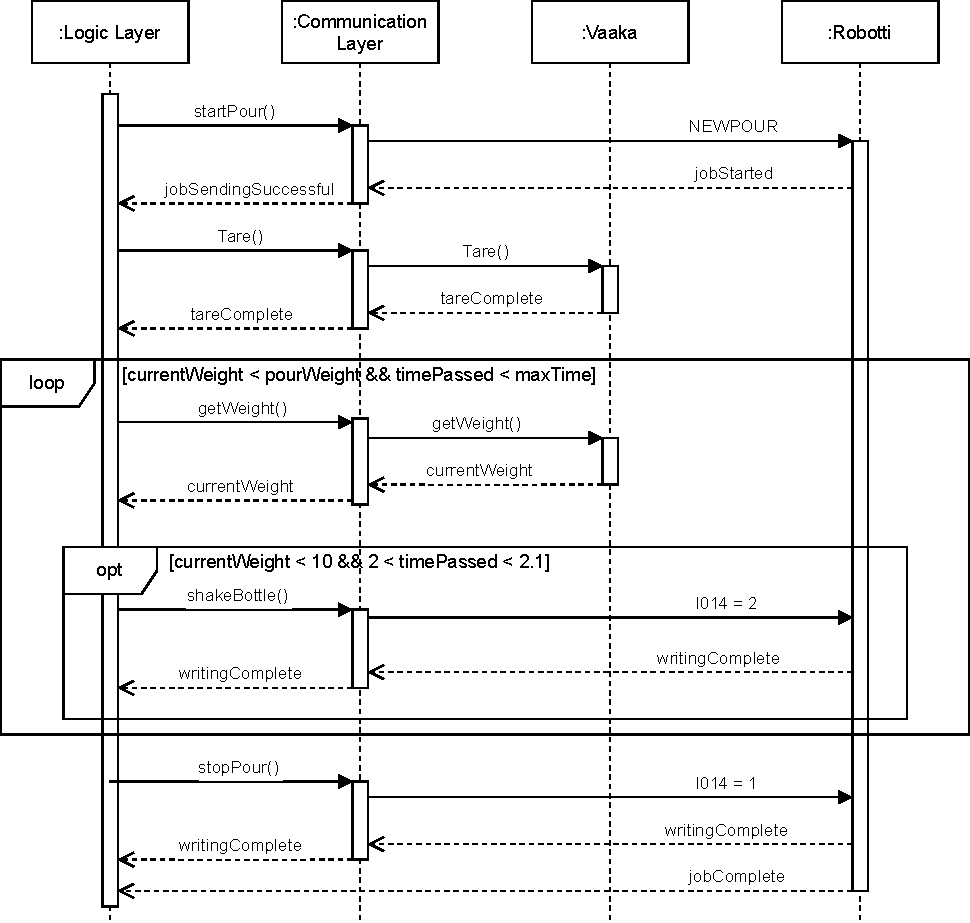
\includegraphics[scale=0.8]{img/sequence.pdf}   %0.8 scale
\end{center}
\caption{Sekvenssikaavio uudesta kaatosysteemistä}
\label{fig:Sequence}
\end{figure}

Yllä olevassa sekvenssikaaviossa kuvassa \ref{fig:Sequence} on havainnollistettu UML-kielellä uuden kaatosysteemin toimintaa.
